\documentclass[aspectratio=169]{beamer}
% --------------------------------------------------
% Opções para "aspectratio"
% 43 ou 54: Formatos 4:3 ou 5:4 tradicionais para telas antigas
% 169, 1610 ou 189: Formatos 16:9, 16:10 ou 18:9 widescrenn telas mais modernas
% --------------------------------------------------
\usepackage{ifslides2024} % Tema (não remover)
\usepackage{lipsum}       % Gerador de texto dummy
\usepackage{csquotes}
\usepackage[utf8]{inputenc}

\addbibresource{referencias.bib} % Referências
% Dados da Apresentação
\vspace*{0.2cm}
\titulo{ ANÁLISE COMPARATIVA ENTRE ALGORITMOS DE PREDIÇÃO DE PREÇO PARA O BITCOIN}
\subtitulo{Seminário de Qualificação de TCC}
\autor{Mickael Osvaldo de Oliveira}
\email{mickaelosvaldo1999@gmail.com}
\info{% Informações adicionais (opcional)
  Bacharelado em Engenharia de Computação \\%
  \textbf{Orientador:} Prof. Dr. Ciniro Aparecido Leite Nametala \\% 
}
\campus{Bambuí}
\data{2024}

\begin{document}

% Página inicial
\begin{frame}[plain, fragile]
  \titlepage
\end{frame}

% ------------------------------------------------------------

% Sumário
\begin{frame}[fragile]{Sumário}
  \tableofcontents
\end{frame}

% ------------------------------------------------------------

\section{Introdução}

\begin{frame}[plain,fragile,t] \frametitle{Introdução}
	\begin{center}
		Contextualização do tema, objetivos e justificativa da pesquisa.
	\end{center}
\end{frame}

% ------------------------------------------------------------

\subsection{Contextualização}

\begin{frame}[fragile] \frametitle{Introdução -- Contextualização}
	\begin{itemize} \itemsep1em
	\item 	A predição de preços em ativos financeiros teve sua origem atribuída a \textcite{Bachelier}, na teoria conhecida como \textit{Random Walks} \cite{Fama1965,Fama};
		
	\item 	Desde então, diversos métodos foram empregados com esse fim, destacando-se a análise técnica, fundamentalista e a utilização de modelos estatísticos como o ARIMA \cite{Ariyo} ou aprendizado de máquina \cite{Fer};
		
	\item 	Com advento da \textit{Blockchain} e \textit{Bitcoin} por \cite{Nakamoto}, um novo mercado de ativos descentralizados surgiu, trazendo consigo a necessidade de novas abordagens de predição de preços \cite{Zhang}.
	\end{itemize} \itemsep1em
\end{frame}

% ------------------------------------------------------------

\subsection{Objetivos}

\begin{frame}[fragile] \frametitle{Introdução -- Objetivos}
\begin{block}{Objetivo Geral}
  Analisar por meio comparativo o desempenho de algoritmos de predição de
preço no contexto do \textit{Bitcoin}.
\end{block}
\vskip1em
\begin{block}{Objetivos Específicos}
  \begin{enumerate}
    \item Desenvolver a estrutura computacional necessária para selecionar, implementar
    e realizar previsões por meio de ferramentas tecnológicas adequadas;
    
    \item Validar de algoritmos de redes neurais e compará-los, frente aos Benchmarks de interesse, a fim de determinar qual tem melhor desempenho;

    \item Explorar de possíveis variações em métodos conhecidos, visando adaptá-los a um novo cenário;
  
    \item Analisar se esses métodos de predição são rentáveis em uma base de dados real.

  \end{enumerate}
\end{block}
\end{frame}

% ------------------------------------------------------------

\subsection{Justificativa}

\begin{frame}[fragile] \frametitle{Introdução -- Justificativa}
	\begin{enumerate}

    \item Os criptoativos tem se tornado uma alternativa ao mercado financeiro tradicional, principalmente devido a sua volatilidade, tem sido adotado como ativo de alto risco \cite{Sousa};
			
		\item Esta pesquisa busca comparar algorítmos de predição de preços, sejam estatísticos ou de aprendizado de máquina, a fim de avaliar seu desempenho em uma base de dados real;
			
		\item As tecnologias convergem para um cenário onde a análise de dados é cada vez mais importante, a inteligência artificial e a rede distribuída são a parte central da Web3;
		
    \item Os modelos utilizados serão o ARIMA, LSTM, BiLSTM e GRU. Em que todas as implementações estarão públicas no GitHub.
		
    \end{enumerate}
\end{frame}

% ------------------------------------------------------------

\section{Fundamentação Teórica}

\begin{frame}[plain,fragile,t] \frametitle{Fundamentação Teórica}
	\begin{center}
		Revisão bibliográfica e fundamentos conceituais necessários para o desenvolvimento do tema.
	\end{center}
\end{frame}

% ------------------------------------------------------------



% ------------------------------------------------------------

\subsection{Fundamentos conceituais}

\begin{frame}[fragile] \frametitle{Fundamentação Teórica -- Fundamentos conceituais}
	\begin{itemize} \itemsep1em
		\item A ideia de Ativos Digitais descentralizados baseados em criptografia, ou criptomoedas, foi marcada por inúmeras tentativs anteriores, mas só foi implementada como advento da \textit{Blockchain} por \cite{Nakamoto} \cite{Moi};
		\item O ARIMA (Autoregressive Integrated Moving Average) tem suas raízes na econometria e na estatística. Sua história remonta ao trabalho pioneiro de \textcite{Box};
		\item A teoria de Redes Neurais Artificiais teve início com os estudos de \textcite{Rosenblatt}, evoluiu com \textcite{Rumelhart}. Atualmente, é associada ao aprendizado profundo proposto por \textcite{Good}.
	\end{itemize}
\end{frame}

\subsection{Revisão Bibliográfica}
\begin{frame}[fragile] 
    \frametitle{Fundamentação Teórica -- Revisão Bibliográfica}
    \begin{columns}[c]
		\begin{column}{1\linewidth}
			\begin{figure}
				\fbox{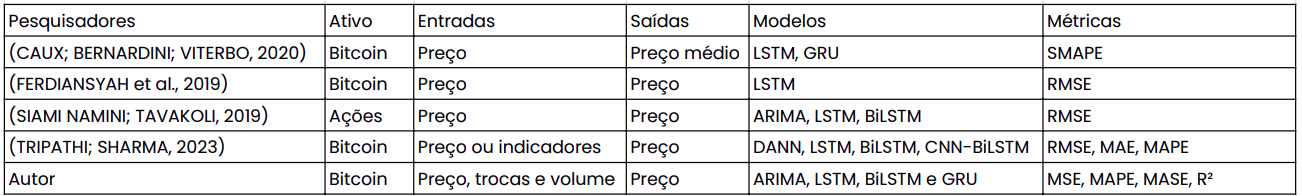
\includegraphics[scale=0.3]{figuras/estudos.png}}
				\label{fig:estudos}
			\end{figure}

			\begin{block}{Estudos similares}
				Tabela contendo os principais estudos relacionados ao tema. Fonte: Próprio autor.    
			\end{block}
		\end{column}
	\end{columns}
\end{frame}

% ------------------------------------------------------------

\section{Metodologia}

\begin{frame}[plain,fragile,t] \frametitle{Metodologia}
	\begin{center}
		Seção destinada a explicar como a pesquisa será realizada.
	\end{center}
\end{frame}

% ------------------------------------------------------------

\subsection{Classificação da pesquisa}

\begin{frame}[fragile] \frametitle{Metodologia -- Classificação da pesquisa}
	\begin{enumerate}
		\item Pode-se dizer, segundo a abordagem de \textcite{pesquisa}, que a pesquisa adota uma abordagem quantitativa e experimental;
		
		\item A natureza aplicada do
    estudo busca não apenas compreender as nuances de cada algoritmo, mas também oferecer
    insights para a seleção e implementação dos mais eficazes;
		
		\item A metodologia descritiva permite
    uma análise detalhada dos resultados obtidos, destacando as diferenças significativas entre
    os modelos avaliados.
	\end{enumerate}
\end{frame}

% ------------------------------------------------------------

\subsection{Solução proposta}
\begin{frame}[fragile]
	\frametitle{Metodologia -- Solução proposta}
		\begin{columns}[c]
			\begin{column}{1\linewidth}
				\begin{figure}
					\fbox{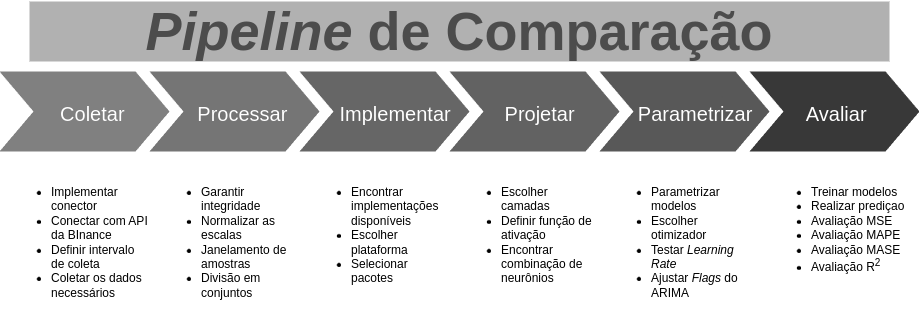
\includegraphics[scale=0.4]{figuras/proposta.png}}
					\label{fig:proposta}
				\end{figure}

				\begin{block}{Fluxo de comparação dos algoritmos}
					Imagem ilustrativa dos passos para a comparação dos algoritmos. Fonte: Próprio autor.    
				\end{block}
			\end{column}
		\end{columns}
	\end{frame}

% ------------------------------------------------------------

\section{Resultados}

\begin{frame}[plain,fragile,t] \frametitle{Resultados}
	\begin{center}
		Resultados parciais encontrados no desenvolvimento da pesquisa.
\end{center}
\end{frame}

\begin{frame}[fragile] \frametitle{Resultados}
	\begin{enumerate}
		\item Ainda é inviável apresentar resultados, pois apesar da metodologia estar pronta, a pesquisa ainda não foi integralmente concluída;
		
		\item Todos os dados foram coletados, sendo obtidas 35136 observações de preços;
		
		\item As métricas de avaliação dos modelos foram definidas, sendo elas: \textit{Mean Squared Error} (MSE), \textit{Mean Absolute Scaled Error} (MASE), \textit{Mean Absolute Percentage Error} (MAPE) e \textit{R-squared} ${R^2}$.
	\end{enumerate}
\end{frame}

\section{Conclusões}

\begin{frame}[plain,fragile,t] \frametitle{Conclusões}
	\begin{center}
		Conclusões e próximos passos.
\end{center}
	
\end{frame}

% ------------------------------------------------------------

\begin{frame}[fragile] \frametitle{Conclusões}
	\begin{enumerate}
		\item A abordagem adotada para a implementação e avaliação dos algoritmos tem se mostrado
		adequada para os objetivos propostos;
		
		\item A continuidade dos experimentos restantes são
	cruciais para validar os resultados e fornecer uma análise mais aprofundada.
	\end{enumerate}
\end{frame}

% ------------------------------------------------------------

\begin{frame}[fragile] \frametitle{Próximos passos}
	\begin{itemize} \itemsep1em
		\item Definir a arquitetura dos modelos a serem utilizados;
		\item Validar os parâmetros das redes e ARIMA;
		\item Implementar janelamento para a comparação.
	\end{itemize}
\end{frame}

\section{Referências}

\begin{frame}[allowframebreaks] 
\frametitle{Referências}
  \printbibliography 
\end{frame}

\begin{frame}[fragile,plain] \frametitle{Obrigado}
\begin{center}
 \vspace*{2em}

 Favor enviar as sugestões e os pedidos de correção para:

 mickaelosvaldo1999@gmail.com 
 
 ciniro.nametala@ifmg.edu.br.

 \vspace*{2em}
 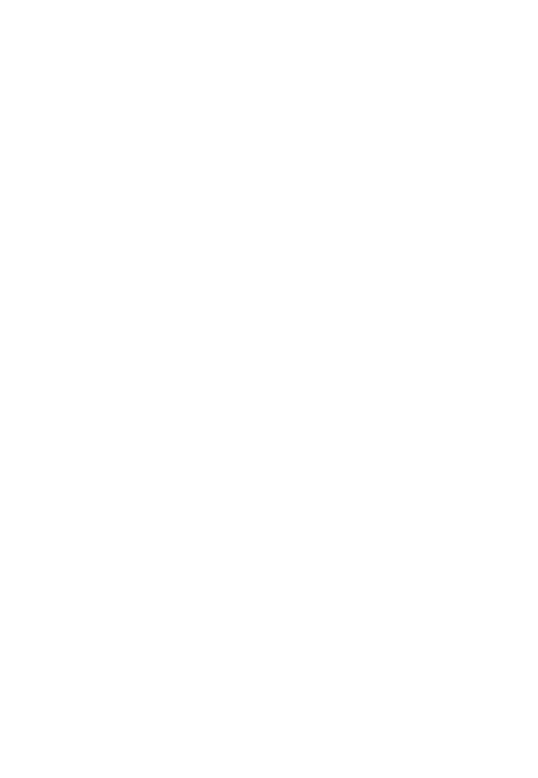
\includegraphics[width=1.5cm]{logoif}
\end{center}
\end{frame}

\end{document}
